\section{Vergleich von Aggregationsmethoden}
    \label{sec:vergleich_aggregationsmethoden}
    % \subsection{Dempster-Shafer-Evidenztheorie}
    % \subsection{Fuzzy-basierte Fusion}
    % \subsection{Bayes-basierte Konsensmodelle}
    % \subsection{Gewichtetes Voting}
    Nun, da jeder Knoten automatisiert einen umfangreichen Threat Report erstellt und eine Vielzahl von Informationen über die Bedrohungslage an seine Nachbarn weitergeben kann, stellt sich die Frage, wie diese Informationen am effektivsten zur verbesserten Erkennung von Angriffen des einzelnen Knotens genutzt werden können. 
    Hierbei ist folgende Problemstellung umfassend zu betrachten:
    
    \begin{itemize}
        \item Jeder Knoten erstellt einen standardisierten Threat Report, wie in Kapitel~\ref{chapter:thread_report} (Konzeption des Threat Reporters) beschrieben, welcher detaillierte Informationen über die lokale Bedrohungslage enthält.
        \item Die Informationen werden an die Nachbarn in einem Peer-to-Peer-Netzwerk über die Pub/Sub-Infrastruktur weitergegeben, wie in Kapitel~\ref{chapter:systemarchitektur} (Systemarchitektur und Detection Framework) dargelegt. Dies erfolgt in einem festen Intervall von 60 Sekunden.
        \item Für die verbesserte Erkennung stehen jedem einzelnen Knoten zu jedem Intervall eine variable Anzahl an Threat Reports von den Nachbar Knoten zur Verfügung. Dies ist dem dynamischen Aufbau der Netzwerktopologie sowie potenziellen Latenzen geschuldet.
        \item Es gilt, eine Methode zu entwickeln, welche die Relevanz der einzelnen Knoten bewertet und somit die Gewichtung der Informationen jedes einzelnen Threat Reports dynamisch und intelligent anpasst.
    \end{itemize}

    \begin{figure}[H]
        \centering
        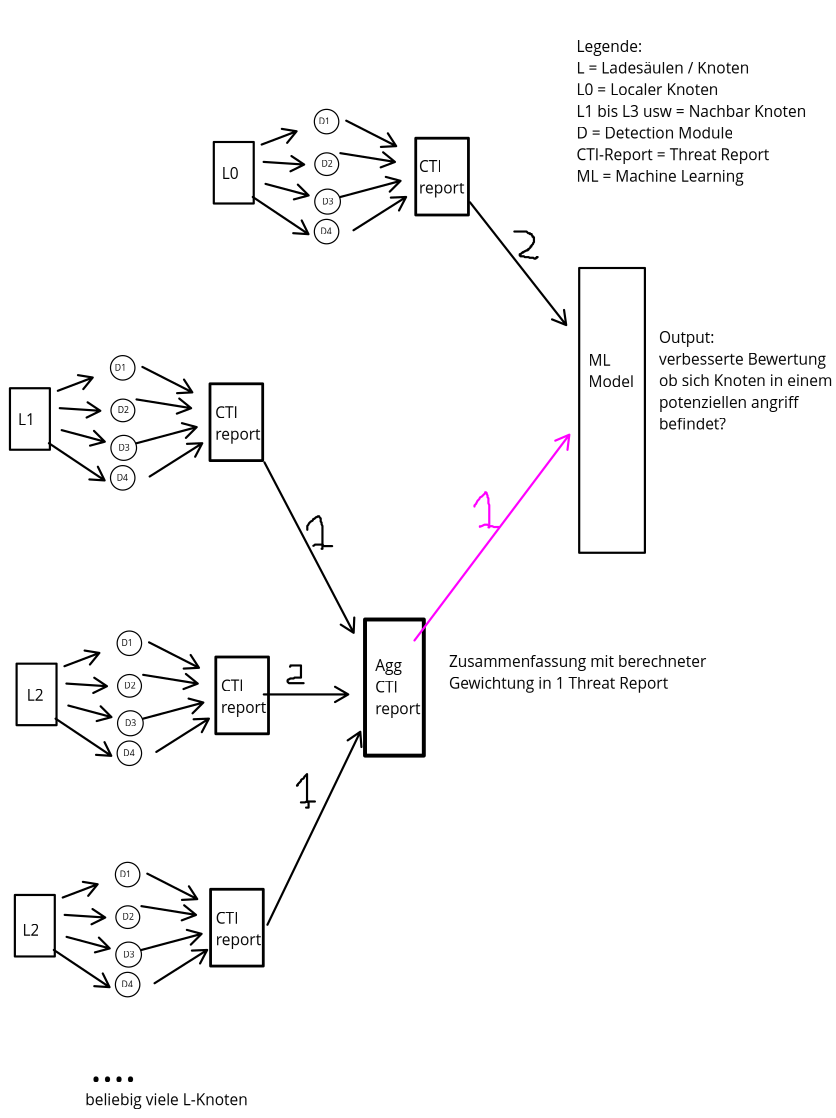
\includegraphics[width=0.75\textwidth]{./figures/Fusions_architektur.png}
        \caption{Aufbau der Fusion von Threat Reports aus Nachbar Knoten}
        \label{fig:aggregation_comparison}
    \end{figure}

    Eine zentrale Herausforderung bei der Verwendung von Machine-Learning-Verfahren, insbesondere bei klassischen neuronalen Netzen, besteht darin, dass diese in der Regel eine Eingabe mit fester Dimension (Fixed-Size Input) benötigen \cite{zaheer2017deepsets}. Da die Anzahl der empfangenen Threat Reports jedoch pro Zeitintervall schwankt, kann keine statische Eingabeschicht definiert werden. Im Folgenden werden daher verschiedene Methoden untersucht, die in der Lage sind, mit dieser Variabilität umzugehen und eine konsistente Datenbasis für das Training und die Inferenz eines Machine-Learning-Modells sicherzustellen.

    \subsection{Statische Aggregation}

    Bei der statischen Aggregation liegt der Fokus auf vorab manuell definierten Regeln. Diese sind regelbasiert konzipiert und verfügen über keine lernenden Komponenten. Ein typisches Szenario für diesen Ansatz ist die situationsbezogene Aggregation: Hierbei werden unterschiedliche Alerts nur dann zu einer Situation konsolidiert, wenn sie dieselbe Quelle, dasselbe Ziel und dieselbe Angriffsklasse aufweisen. Die Granularität dieser Zusammenfassung wird dabei durch statisch konfigurierte Schwellenwerte gesteuert \cite{debar2001aggregation}. Als gängige mathematische Aggregationsmethoden kommen in diesem Kontext nach der Gruppierung die Berechnung von Minimum, Maximum, Durchschnitt oder der Standardabweichung zum Einsatz \cite{lee2019settransformer, liu2022pooling}.
    
    %%%%%%%%%%%%%%%%%%%%%%%%%%%%%%%%%%%%%%%%%%%%%%%%%%%%%%%%%%%%%%%%%%%%%%%%%%%%%%%%
    \subsection{Padding und Masking}
    \label{subsec:padding_und_masking}

    Padding und Masking sind essenzielle Verfahren bei der Verarbeitung von Sequenzdaten, um die Inferenz mit variierenden Sequenzlängen zu ermöglichen. Diese Mechanismen sind standardmäßig in modernen Deep-Learning-Frameworks integriert, wie beispielsweise im Parameter \texttt{key\_padding\_mask} der \texttt{torch.nn.MultiheadAttention}-Klasse in PyTorch \cite{pytorch2024multihead}.

    Der Prozess des Paddings definiert eine maximale Sequenzlänge $n_{\max}$. Sequenzen, die diese Länge unterschreiten, werden mit speziellen \texttt{[PAD]}-Token aufgefüllt, bis sie die Dimension $n_{\max}$ erreichen. Damit diese künstlich hinzugefügten Token das Training oder die Aggregation nicht verfälschen, wird eine Maskierung (Masking) eingesetzt. Diese stellt sicher, dass die entsprechenden Positionen während der Berechnung der Attention-Scores ignoriert werden.

    In der Arbeit von Vaswani et al. (2017) \cite{vaswani2017attention} bildet dieses Prinzip die Grundlage für die effiziente Batch-Verarbeitung innerhalb der Transformer-Architektur. Hierbei verhindert das Masking, dass das Modell Aufmerksamkeit auf Padding-Bereiche richtet (siehe Abbildung \ref{fig:padding_masking}).

    \begin{figure}[H]
        \centering
        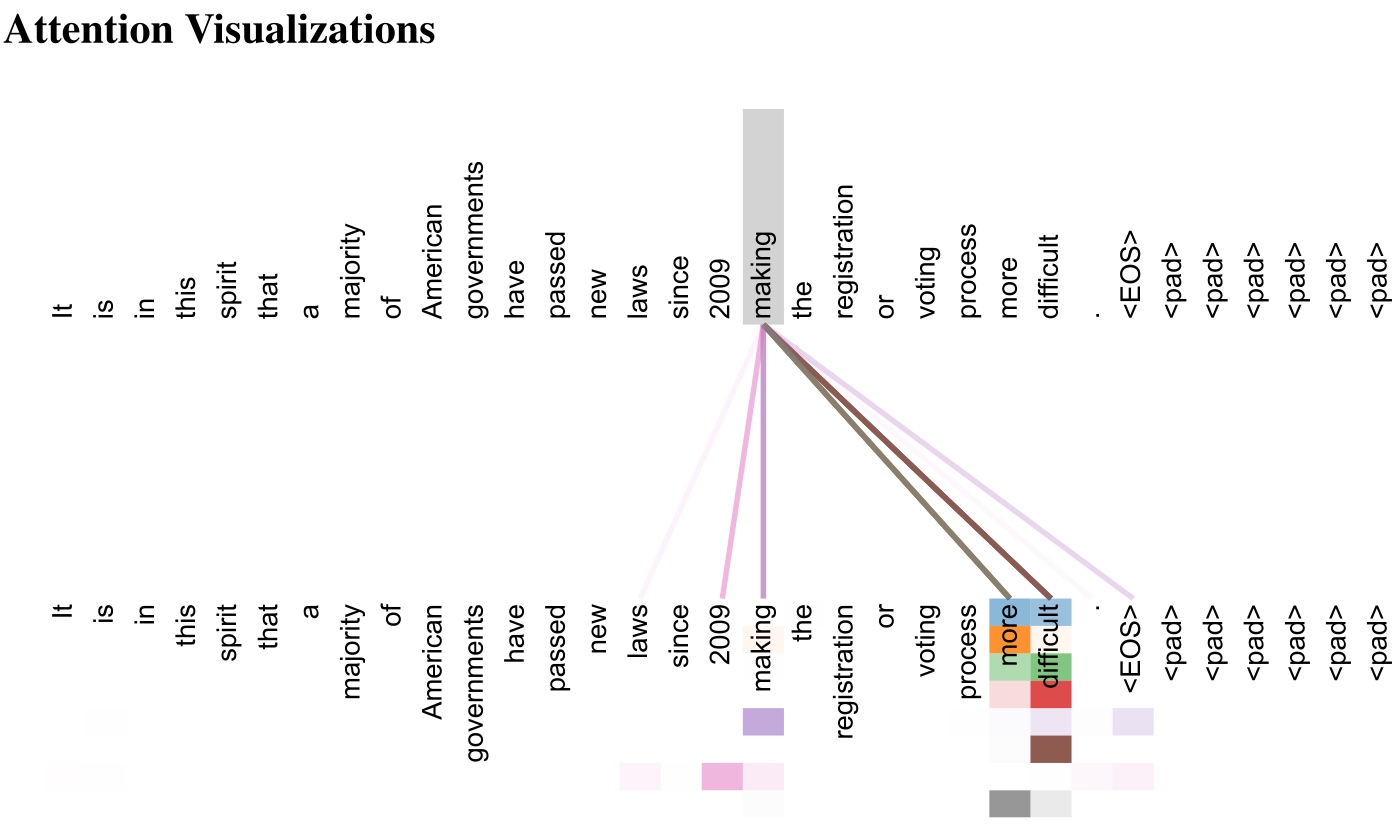
\includegraphics[width=0.75\textwidth]{./figures/masking_attention_is_all_you_need.png}
        \caption{Visualisierung der Attention-Mechanismen (adaptiert nach Figure 3 aus \cite{vaswani2017attention})}
        \label{fig:padding_masking}
    \end{figure}

    Ebenso findet dieses Verfahren Anwendung in der BERT-Architektur von Devlin et al. (2019) \cite{devlin2019bert}. Hierbei werden Eingabesequenzen auf eine feste Länge von meist 512 Token gepaddet, wobei das Masking sowohl für das Padding als auch für die spezifische Trainingsmethode des \textit{Masked Language Modeling} (MLM) verwendet wird.

    %%%%%%%%%%%%%%%%%%%%%%%%%%%%%%%%%%%%%%%%%%%%%%%%%%%%%%%%%%%%%%%%%%%%%%%%%%%%%%%%
    \subsection{Deep Sets}
    \label{subsec:deep_set}
    Im Gegensatz zu den in Abschnitt \ref{subsec:padding_und_masking} beschriebenen Verfahren, die auf einer fixen Anzahl von Elementen basieren, verfolgen \textit{Deep Sets} einen mengenbasierten Ansatz. Dabei wird die Eingabe als eine ungeordnete Menge $X$ betrachtet. Das Modell lernt hierbei, die Relevanz der einzelnen Elemente autonom zu bewerten und die Gewichtung der Informationen dynamisch anzupassen. 

    Eine fundamentale Anforderung an die verarbeitende Funktion $f(X)$ ist die \textit{Permutationsinvarianz}. Dies bedeutet, dass die Ausgabe der Funktion unabhängig von der Reihenfolge der Elemente innerhalb der Menge sein muss \cite{zaheer2017deepsets}.

    \begin{theorem}[Zaheer et al., 2017]
    Eine Funktion $f(X)$ auf einer Menge $X$, deren Elemente aus einem abzählbaren Universum stammen, ist genau dann permutationsinvariant, wenn sie sich wie folgt dekomponieren lässt:
    \[
    f(X) = \rho \left( \sum_{x \in X} \phi(x) \right)
    \]
    wobei $\phi$ und $\rho$ geeignete Transformationen (typischerweise neuronale Netze) darstellen.
    \end{theorem}

    Während die Summenbildung die theoretische Grundlage für die Aggregation bildet, werden in der Praxis häufig auch der Mittelwert (\textit{Mean}) oder das Maximum (\textit{Max}) verwendet, da diese Operationen ebenfalls die Bedingung der Permutationsinvarianz erfüllen. Soelch et al. zeigen jedoch auf, dass die Wahl der Aggregationsfunktion einen erheblichen Einfluss auf die Modellperformance hat, und schlagen als Alternative lernbare Aggregationsmechanismen vor \cite{soelch2019deepsetAgg}.

    %%%%%%%%%%%%%%%%%%%%%%%%%%%%%%%%%%%%%%%%%%%%%%%%%%%%%%%%%%%%%%%%%%%%%%%%%%%%%%%%
    \subsection{Set2Set}
    \label{subsec:set2set}
  
    Obwohl auch Ansätze der vorherigen Aggregationsmethoden variable Eingabelängen verarbeiten können, unterscheiden sie sich von Set2Set primär in der Art der Informationsverdichtung. Während herkömmliche Methoden die Eingabemenge meist durch eine statische Aggregationsfunktion (z. B. Mean-Pooling) in einen fixen Merkmalsraum transformieren, nutzt Set2Set einen iterativen \textit{Read-Process}. Durch die Kombination aus Attention-Mechanismen und einem rekurrenten Zustand kann das Modell die Menge mehrfach explorieren. Dies ermöglicht es, komplexe Abhängigkeiten zwischen den Elementen aufzulösen, die bei einer einfachen Summation oder Mittelwertbildung verloren gingen \cite{vinyals2016orderm}.

    Algorithmische Experimente, wie das Sortieren von Zahlenfolgen, belegen, dass Modelle eine höhere Lern- und Generalisierungsfähigkeit aufweisen, wenn sie nicht durch eine willkürliche Reihenfolge der Eingabedaten eingeschränkt werden \cite{vinyals2016orderm}. Auch die in Abschnitt \ref{subsec:padding_und_masking} behandelten Transformer-Architekturen werden mit einer Form des Set2Set-Ansatzes erweitert \cite{vaswani2017attention}.
    

    %%%%%%%%%%%%%%%%%%%%%%%%%%%%%%%%%%%%%%%%%%%%%%%%%%%%%%%%%%%%%%%%%%%%%%%%%%%%%%%%
    \subsection{Graph Neural Networks and Pooling}
    Graph Neural Networks (GNNs) bieten eine leistungsstarke Methode zur Verarbeitung von Daten, die in Form von Graphen vorliegen. Knoten repräsentieren dabei Entitäten (z.\,B. IP-Adressen), während Kanten die Beziehungen zwischen diesen Entitäten modellieren und die zugehörigen Flow-Informationen als Kantenmerkmale tragen \cite[Sec.\,III-A]{lo2022egraphsage}. 

    Durch iteratives Aggregieren der Nachbarschaftsinformationen können GNNs sowohl topologische Muster als auch merkmalsbasierte Strukturen im Netzwerkgraphen erkennen. Das Pooling erfolgt hier, wie bereits in Abschnitt~\ref{subsec:set2set} beschrieben, mittels Mean-Pooling über die Kanten-Features der Nachbarschaft \cite[Sec.\,IV-A, Eq.\,6]{lo2022egraphsage}.
    %%%%%%%%%%%%%%%%%%%%%%%%%%%%%%%%%%%%%%%%%%%%%%%%%%%%%%%%%%%%%%%%%%%%%%%%%%%%%%%%